% =====================================================================
%  Progress presentation (Beamer, single-file) --- for the supervisor.
%  The modelling half: an honest NEGATIVE result, in plain English.
%  Build:  report/build.sh report/presentation   (Tectonic + Ghostscript-normalise)
% =====================================================================
\documentclass[aspectratio=169,11pt]{beamer}
\usetheme{default}
\setbeamertemplate{navigation symbols}{}
\setbeamertemplate{footline}[frame number]
\setbeamertemplate{itemize items}[circle]

\usepackage{amsmath,amssymb}
\usepackage{booktabs}
\usepackage{tikz}
\usetikzlibrary{positioning,arrows.meta,calc}
\usepackage{pgfplots}
\pgfplotsset{compat=1.18}

% --- self-contained palette (matches the status deck) ---
\definecolor{navy}{RGB}{30,64,124}
\definecolor{forest}{RGB}{34,120,60}
\definecolor{burnt}{RGB}{214,104,26}
\definecolor{plum}{RGB}{140,55,135}
\setbeamercolor{structure}{fg=navy}
\setbeamercolor{frametitle}{fg=navy}
\setbeamerfont{frametitle}{series=\bfseries}

\newcommand{\frozen}[1]{{\color{navy}\textbf{#1}}}
\newcommand{\ck}{{\color{forest}$\checkmark$}}
\newcommand{\no}{{\color{burnt}\textbf{--}}}

\title[Progress update]{Predicting the Zero-Shot Transfer of a Promptable Video Tracker}
\subtitle{Progress update --- the modelling half, and an honest \emph{negative} result}
\author{Kostiantyn Boiar}
\institute{MSc Dissertation \,\textbullet\, University of Glasgow\\[2pt]
\small Supervisor: Dr Marwa Mahmoud}
\date{\today}

\begin{document}

% ---------------------------------------------------------------- title
\begin{frame}[plain]
  \titlepage
\end{frame}

% ------------------------------------------------------------ headline
\begin{frame}{The result, in one sentence}
  \begin{block}{}
    \centering\large
    We can \textbf{measure} SAM\,3's reliability --- but we \textbf{cannot predict it in advance} from
    label-free ``distance'' signals, beyond a small and obvious \textbf{animal-size} effect.
  \end{block}
  \vspace{0.6em}
  \begin{itemize}\footnotesize
    \item This is a \textbf{clean, rigorous negative result} --- and it is the contribution.
    \item It is \emph{not} a weak-test artefact: the same test \emph{does} pick up the size effect (shown later).
    \item Everything below is built, tested, and validated out-of-sample with honest statistics.
  \end{itemize}
\end{frame}

% ------------------------------------------------------------ the question
\begin{frame}{The question (plain English)}
  \begin{block}{}
    \centering
    Point SAM\,3 at a video, type ``\texttt{impala}'', and it finds and follows the animal ---
    \textbf{with no training on that species}. Can we tell, \emph{before running it}, whether it will work
    for a \textbf{new animal} in a \textbf{new place} --- \textbf{without labelling anything first}?
  \end{block}
  \vspace{0.5em}
  \centering
  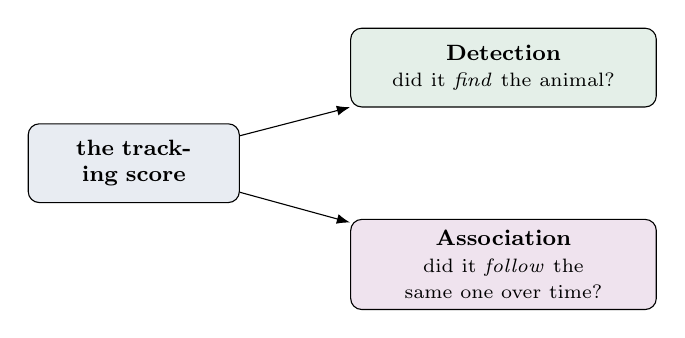
\begin{tikzpicture}[>=Latex,
    box/.style={draw,rounded corners,align=center,font=\footnotesize,inner sep=4pt,minimum height=1cm}]
    \node[box,fill=navy!10,text width=2.4cm] (h) {\textbf{the tracking score}};
    \node[box,fill=forest!12,text width=3.6cm,above right=0.2cm and 1.4cm of h] (d)
        {\textbf{Detection}\\\scriptsize did it \emph{find} the animal?};
    \node[box,fill=plum!14,text width=3.6cm,below right=0.2cm and 1.4cm of h] (a)
        {\textbf{Association}\\\scriptsize did it \emph{follow} the same one over time?};
    \draw[->] (h) -- (d); \draw[->] (h) -- (a);
  \end{tikzpicture}\\[2pt]
  {\footnotesize We split the question in two --- that split is the intellectual core of the project.}
\end{frame}

% ------------------------------------------------------------ what we've done
\begin{frame}{What we've done}
  \begin{enumerate}\footnotesize
    \item \ck\ \textbf{Measured the model.} Ran frozen SAM\,3 over the test videos and scored it with the
          \emph{official} evaluator --- a reliability number for each (species, place, time) group.
    \item \ck\ \textbf{Built four ``distance'' signals} --- how \emph{different} a new species/place is from the
          familiar training data: the animal (tree-of-life $+$ appearance), the scene, and the time gap.
    \item \ck\ \textbf{Fitted a proper model} (score $=$ function of the distances) and tested it
          \textbf{honestly out-of-sample}: hide whole species and whole places, predict them, compare to the
          truth --- with conservative, group-aware error bars.
    \item \ck\ \textbf{Tried a second idea} when the first failed --- maybe it is how \emph{hard} the footage
          is (dark/night, cluttered, small animal), not how \emph{novel} it is.
    \item \ck\ \textbf{Checked a side question} --- when the animal is \emph{absent}, does the model
          hallucinate one?
  \end{enumerate}
\end{frame}

% ------------------------------------------------------------ the null (chart)
\begin{frame}{The main result: the distances predict \emph{nothing}}
  \begin{columns}[T]
    \begin{column}{0.52\textwidth}
      \centering
      \footnotesize
      \begin{tabular}{lcc}
        \toprule
        Predict from & error & beats ``guess''? \\
        \midrule
        guess the average  & $0.298$ & --- \\
        $+$ four distances & $0.298$ & \no\ \textbf{no} \\
        $+$ animal size    & $0.281$ & \ck\ a little \\
        \bottomrule
      \end{tabular}\\[8pt]
      {\scriptsize out-of-sample error $\cdot$ held-out species / places \\ (lower is better)}
    \end{column}
    \begin{column}{0.48\textwidth}
      \begin{itemize}\footnotesize
        \item Hide a species (or a place) and predict it from the distances $\to$ \textbf{no better than
              simply guessing the average}.
        \item Every distance's effect is \textbf{statistically indistinguishable from zero}, on \emph{both}
              hold-out schemes.
        \item The only thing that moves the needle at all is \textbf{animal size} --- and only a little.
      \end{itemize}
    \end{column}
  \end{columns}
\end{frame}

% ------------------------------------------------------------ the size confound
\begin{frame}{The one ``signal'' was a trick of animal size}
  \begin{itemize}\footnotesize
    \item One distance (\textbf{visual}) looked significant --- but with the \emph{wrong} sign, and it was a
          \textbf{confound}: ``visually distinctive species do better'' really means ``\textbf{bigger animals
          are easier to spot}.''
    \item Add an animal-size control and the effect \textbf{vanishes} (coefficient $+0.37 \to +0.22$, now
          overlapping zero); size itself is the real driver.
  \end{itemize}
  \vspace{0.4em}
  \begin{block}{The ``difficulty'' idea collapsed the same way}
    \footnotesize
    Dark / cluttered footage \emph{looked} predictive --- but only because it tracks animal size. On its own it
    predicts nothing (a strong-looking $r\!=\!-0.38$ across places shrinks to $-0.13$ per clip: a classic
    grouping illusion). \textbf{The difficulty pivot is also a null.}
  \end{block}
\end{frame}

% ------------------------------------------------------------ decomposition table
\begin{frame}{Peeling it apart: only \emph{size} survives}
  \centering
  \begin{table}
  \scriptsize
  \begin{tabular}{lcc}
    \toprule
    Predict detection from\dots & Beats guessing? & Gain \\
    \midrule
    clip length only          & \no\ no              & $\approx 0$ \\
    \textbf{animal size} only & \ck\ \textbf{yes}    & $+0.017$ \\
    low-light only (no size)  & \no\ no              & $+0.004$ (n.s.) \\
    low-light $+$ size        & \ck\ yes ($=$ size)  & $+0.020$ \\
    \bottomrule
  \end{tabular}
  \end{table}
  \vspace{0.4em}
  \begin{itemize}\footnotesize
    \item Size \textbf{alone} carries the whole gain; low-light \textbf{alone} does not validate.
    \item So the \emph{only} label-free property that predicts detection is \textbf{object size} --- small,
          obvious, and the very thing we introduced as a \textbf{nuisance control}.
  \end{itemize}
\end{frame}

% ------------------------------------------------------------ association
\begin{frame}{``Following'' barely differs from ``finding''}
  \begin{itemize}
    \item Almost every clip has a \textbf{single animal}, so the two scores are nearly identical
          --- they agree about \textbf{94\%} of the time.
    \item There is very little separate ``following'' signal for \emph{any} feature to predict.
    \item So the association half is honestly a \textbf{detection story}; we report its null with those
          numbers as the explanation, not as a separate failed search.
  \end{itemize}
  \vspace{0.4em}
  \begin{block}{}
    \centering\footnotesize The detection-vs-association split was the right question to ask ---
    the honest finding is that, on this data, association carries almost no distinct signal.
  \end{block}
\end{frame}

% ------------------------------------------------------------ positive control
\begin{frame}{Is ``we found nothing'' trustworthy?}
  \begin{block}{The obvious worry}
    \centering\footnotesize \emph{``Maybe the test just isn't sensitive enough.''}
  \end{block}
  \vspace{0.4em}
  \begin{itemize}
    \item The \textbf{same test}, on the \textbf{same data}, \emph{does} detect the animal-size effect
          out-of-sample.
    \item A test that \textbf{fires for size} but \textbf{stays flat for the distances} is genuinely finding
          \emph{no signal} --- not failing to look.
  \end{itemize}
  \vspace{0.3em}
  \begin{block}{}
    \centering \textbf{This is the key defence of the negative result.}
  \end{block}
\end{frame}

% ------------------------------------------------------------ two extras
\begin{frame}{Two other things we checked}
  \begin{block}{Hallucinations (animal absent)}
    \footnotesize
    SAM\,3 wrongly returns an animal about \textbf{10\%} of the time. More distinctive species hallucinate
    \emph{less} (a real, size-independent correlation) --- but out-of-sample it \textbf{just misses}
    significance ($p=0.053$). A genuine correlation, \textbf{not} a validated predictor.
  \end{block}
  \vspace{0.3em}
  \begin{block}{The model's own confidence (explored, then set aside)}
    \footnotesize
    If we let SAM\,3 \emph{run first} and read its own confidence, that \emph{does} predict its accuracy.
    We deliberately keep it out of the contribution: (1) it needs running the model, defeating the
    ``predict \emph{before} running'' goal; and (2) it is near-circular (a known result). We use it only as an
    internal check that the pipeline can detect a strong signal.
  \end{block}
\end{frame}

% ------------------------------------------------------------ why it matters
\begin{frame}{Why a negative result is a real contribution}
  \begin{itemize}
    \item \textbf{First of its kind:} no one has asked this for a promptable video \emph{tracker}, or split it
          into detection vs association --- novel regardless of the answer.
    \item \textbf{Useful for practitioners:} ``far-from-training'' does \emph{not} mean ``unreliable,'' so
          conservation teams should \textbf{not} trust distance-from-training as a safety check ---
          spot-audit with a few labels instead.
    \item \textbf{Stronger than a weak positive:} a robust null from a demonstrably powerful test is more
          defensible than a borderline effect scraped past a threshold.
  \end{itemize}
\end{frame}

% ------------------------------------------------------------ status / next
\begin{frame}{Where we are, and what's next}
  \begin{block}{Done \& validated}
    \centering\footnotesize
    Measurement \ck\;\; four distances \ck\;\; modelling $+$ out-of-sample validation \ck\;\;
    difficulty pivot \ck\;\; write-up drafted \ck
  \end{block}
  \vspace{0.5em}
  \begin{itemize}\footnotesize
    \item \textcolor{burnt}{\textbf{Writing up}} --- results and discussion now reflect the negative result
          and its explanation.
    \item \textbf{Honest limitation:} distances are to the \emph{dataset's} training split, not SAM\,3's true
          (undisclosed) training data --- a proxy for that is a possible future angle.
    \item \textbf{Possible next direction:} probe whether SAM\,3's own internal features already ``know'' a
          species.
  \end{itemize}
  \vspace{0.3em}
  \centering\small\color{navy}\textbf{Thank you --- questions welcome.}
\end{frame}

\end{document}
